\documentclass{beamer}

\usepackage[utf8]{inputenc}
\usepackage[frenchb]{babel}
\usepackage{verbatim}
\usepackage{graphicx}
\usepackage{color}
\usepackage{hyperref}
\usepackage{url}
\usepackage{moreverb}
\usepackage{fancyvrb}
\usepackage{natbib}
\usepackage{eulervm}
\usepackage{auto-pst-pdf}
\usepackage{pst-plot}
\usepackage{multirow}


\hypersetup{colorlinks=true, linkcolor=black, urlcolor=blue}
\usetheme{boxes}
\beamertemplatenavigationsymbolsempty
\setbeamertemplate{sections/subsections in toc}[circle]
\setbeamertemplate{footline}[frame number]
\setbeamertemplate{itemize items}[circle]
\setbeamertemplate{itemize subitem}[square]

\title{{\bf Scikit-Learn in particle physics}}
\author{Gilles Louppe}
\institute{CERN, Switzerland}
\date{November 18, 2014}

\newcommand{\todo}[1]{\textcolor{red}{[TODO] #1}}

\definecolor{lightgreen}{rgb}{0.0,0.8,0.0}
\definecolor{lightblue}{rgb}{0.3,0.8,1.0}
\definecolor{lightred}{rgb}{0.874,0.180,0.105}
\definecolor{gray}{rgb}{0.4,0.4,0.4}
\definecolor{lightgray}{rgb}{0.8,0.8,0.8}
\definecolor{shadecolor}{rgb}{0.9,0.9,0.9}
\newrgbcolor{mygreen}{.00 .5 .00}
\newrgbcolor{myyellow}{.6 .6 .00}

\DeclareMathOperator*{\argmax}{arg\,max}


\newrgbcolor{mygreen}{.00 .5 .00}
\newcommand{\X}[1]{\textcolor{blue}{#1}}
\newcommand{\y}[1]{\textcolor{red}{#1}}
\newcommand{\model}[1]{\textcolor{orange}{#1}}
\newcommand{\loss}[1]{\textcolor{lightblue}{#1}}
\newcommand{\w}[1]{\textcolor{mygreen}{#1}}
\setbeamertemplate{enumerate items}[circle]

\begin{document}


% -----------------------------------------------------------------------------

\begin{frame}
\titlepage
\end{frame}

% -----------------------------------------------------------------------------

{
\usebackgroundtemplate{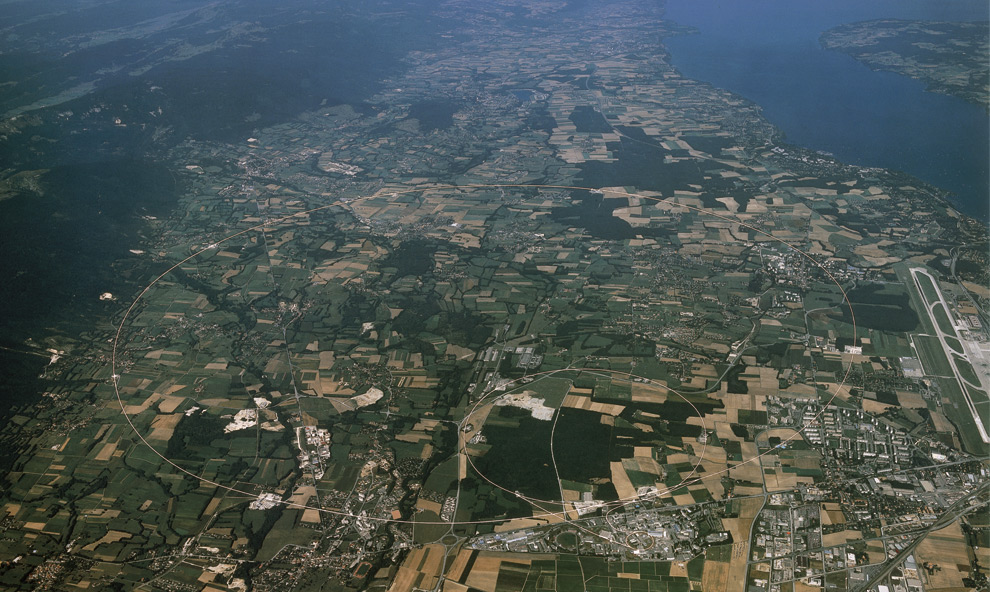
\includegraphics[height=\paperheight]{./figures/lhc.jpg}}
\setbeamercolor{frametitle}{fg=white}
\setbeamercolor{normal text}{fg=white}

\begin{frame}{High Energy Physics (HEP)}

\begin{columns}
    \begin{column}{0.5\textwidth}
    \onslide<3->{
    \begin{figure}
    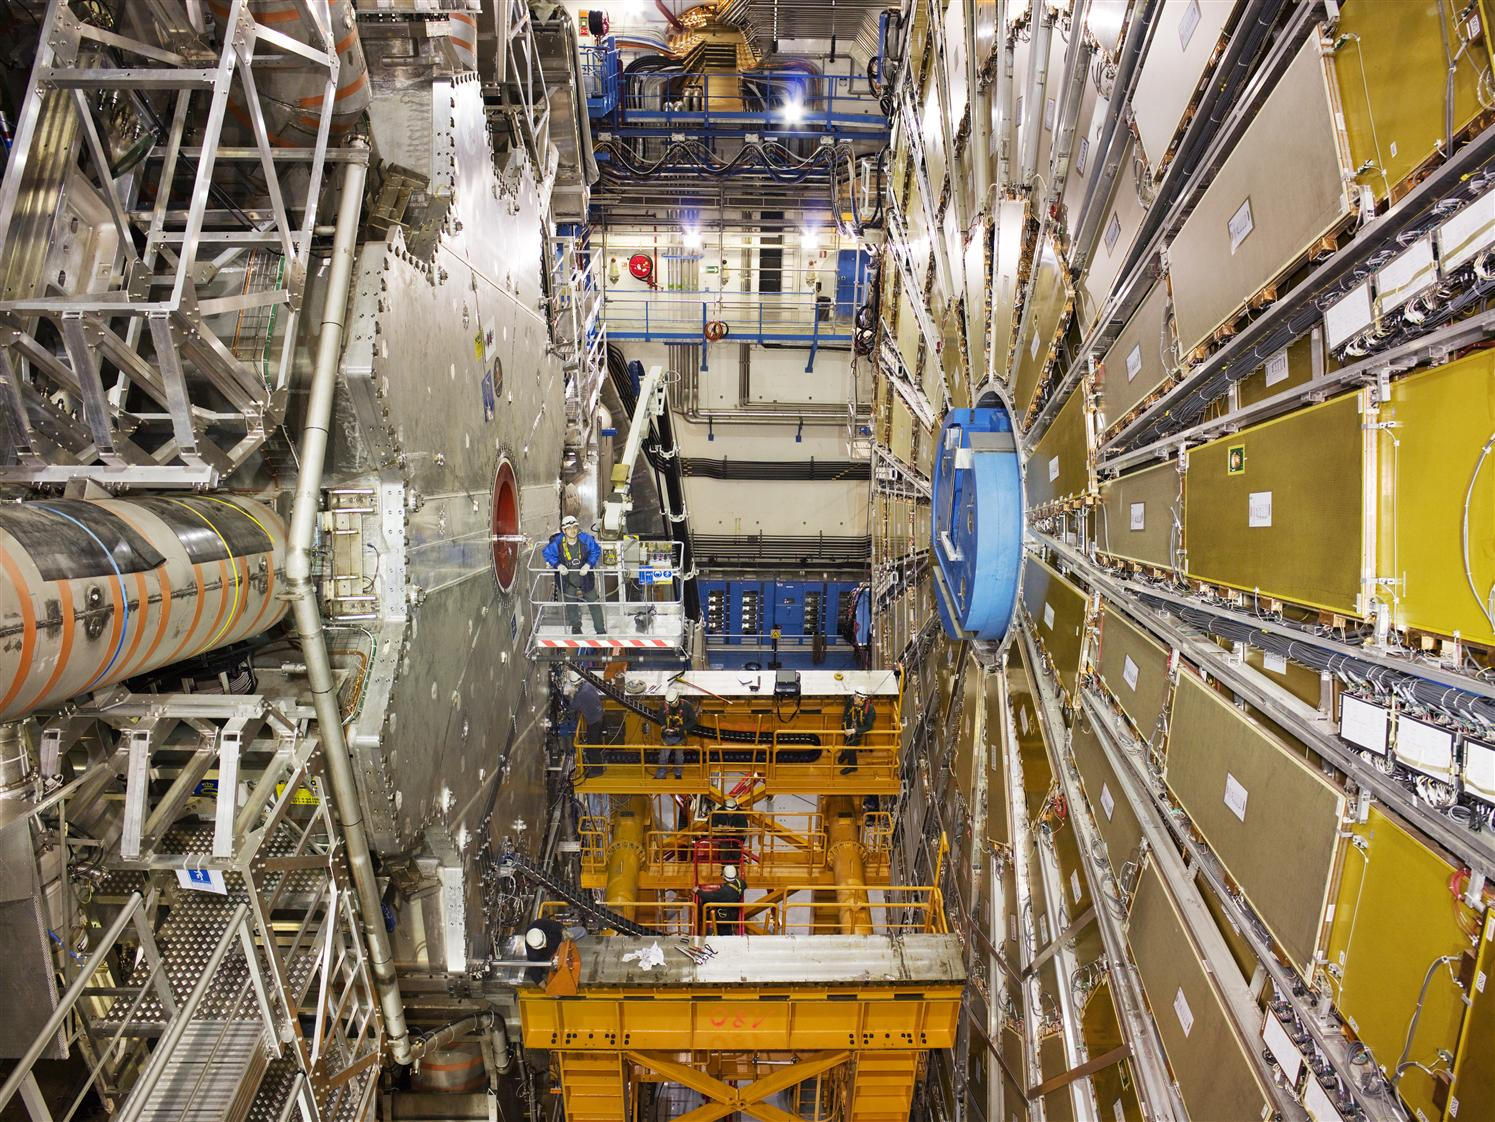
\includegraphics[width=0.8\textwidth]{./figures/atlas.jpg}
    \end{figure}
    \begin{figure}
    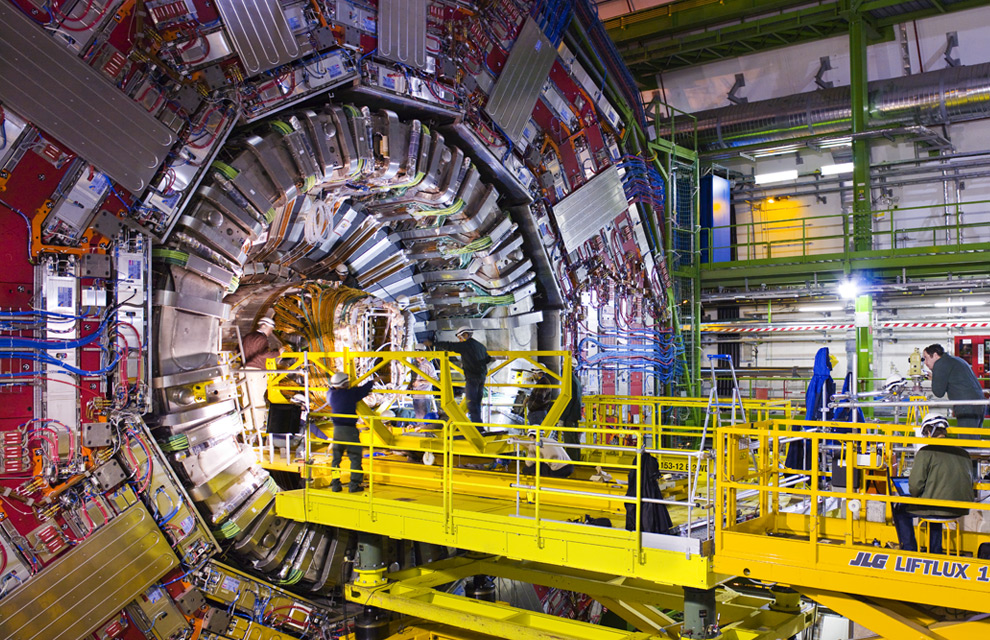
\includegraphics[width=0.8\textwidth]{./figures/cms.jpg}
    \end{figure}}
    \end{column}
    \begin{column}{0.5\textwidth}
    \onslide<2->{
        \begin{center}
        \color{white} \Large \it  Study the nature of the constituents of matter
        \end{center}
    }
    \onslide<3->{
    \begin{figure}
    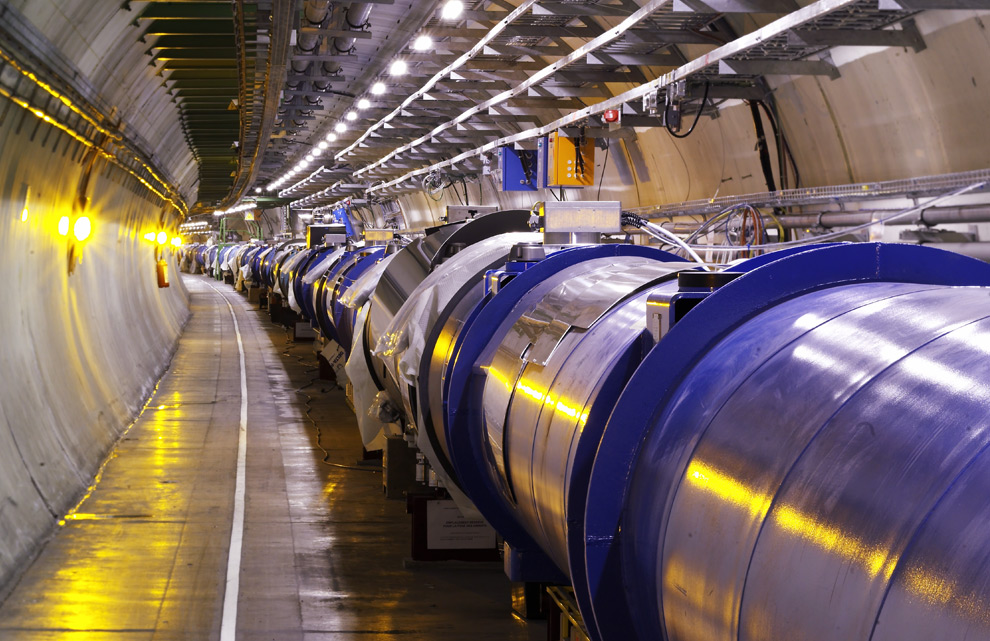
\includegraphics[width=0.8\textwidth]{./figures/tunnel.jpg}
    \end{figure}}
    \end{column}
\end{columns}
\end{frame}
}

% -----------------------------------------------------------------------------

{
\setbeamercolor{frametitle}{fg=white}
\setbeamercolor{normal text}{fg=white}
\setbeamercolor{background canvas}{bg=black}

\begin{frame}{Particle detector 101}
    \only<1>{
        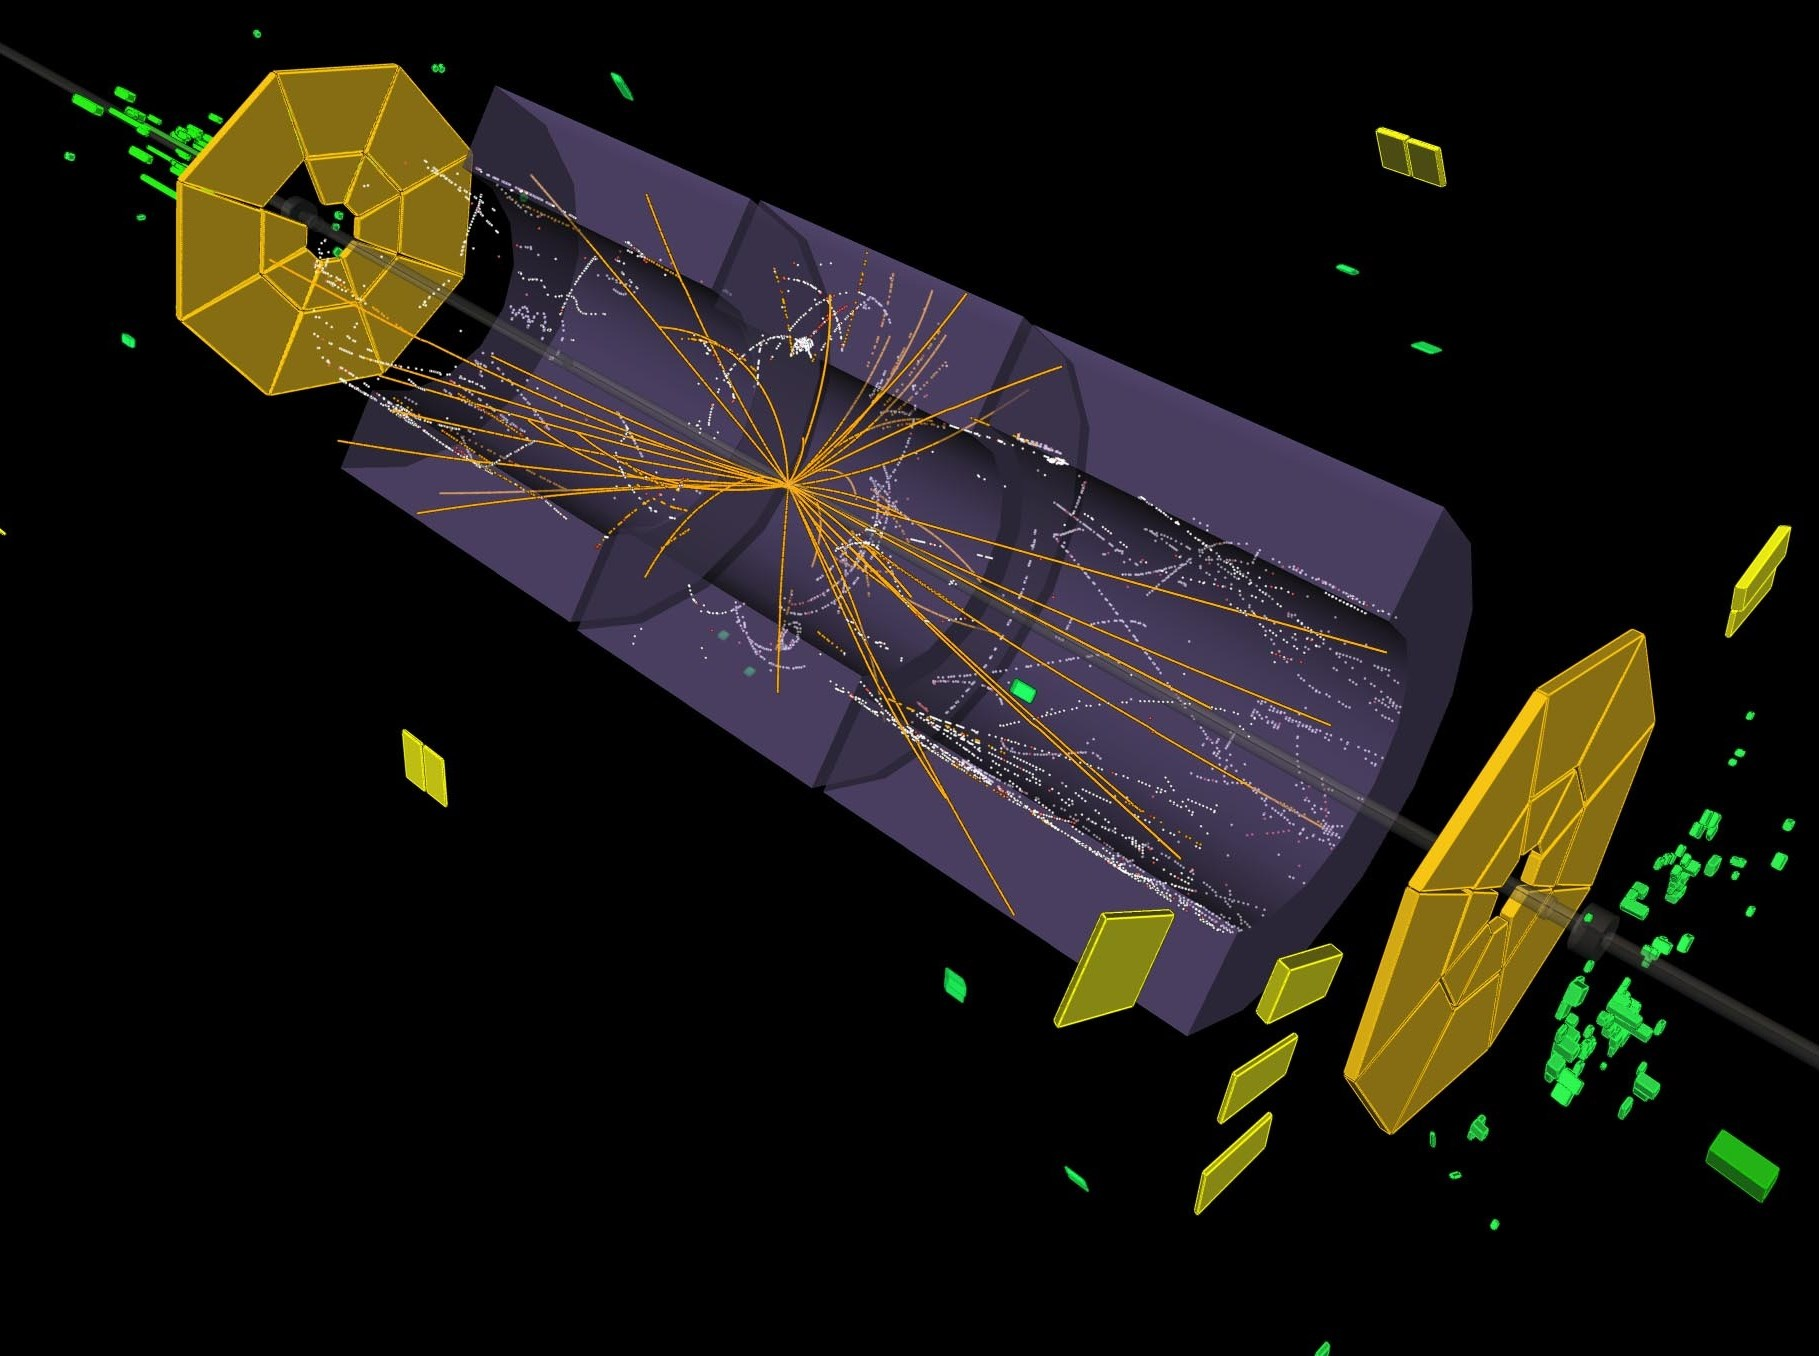
\includegraphics[width=\textwidth]{./figures/collision.jpg}
    }
    \only<2>{
        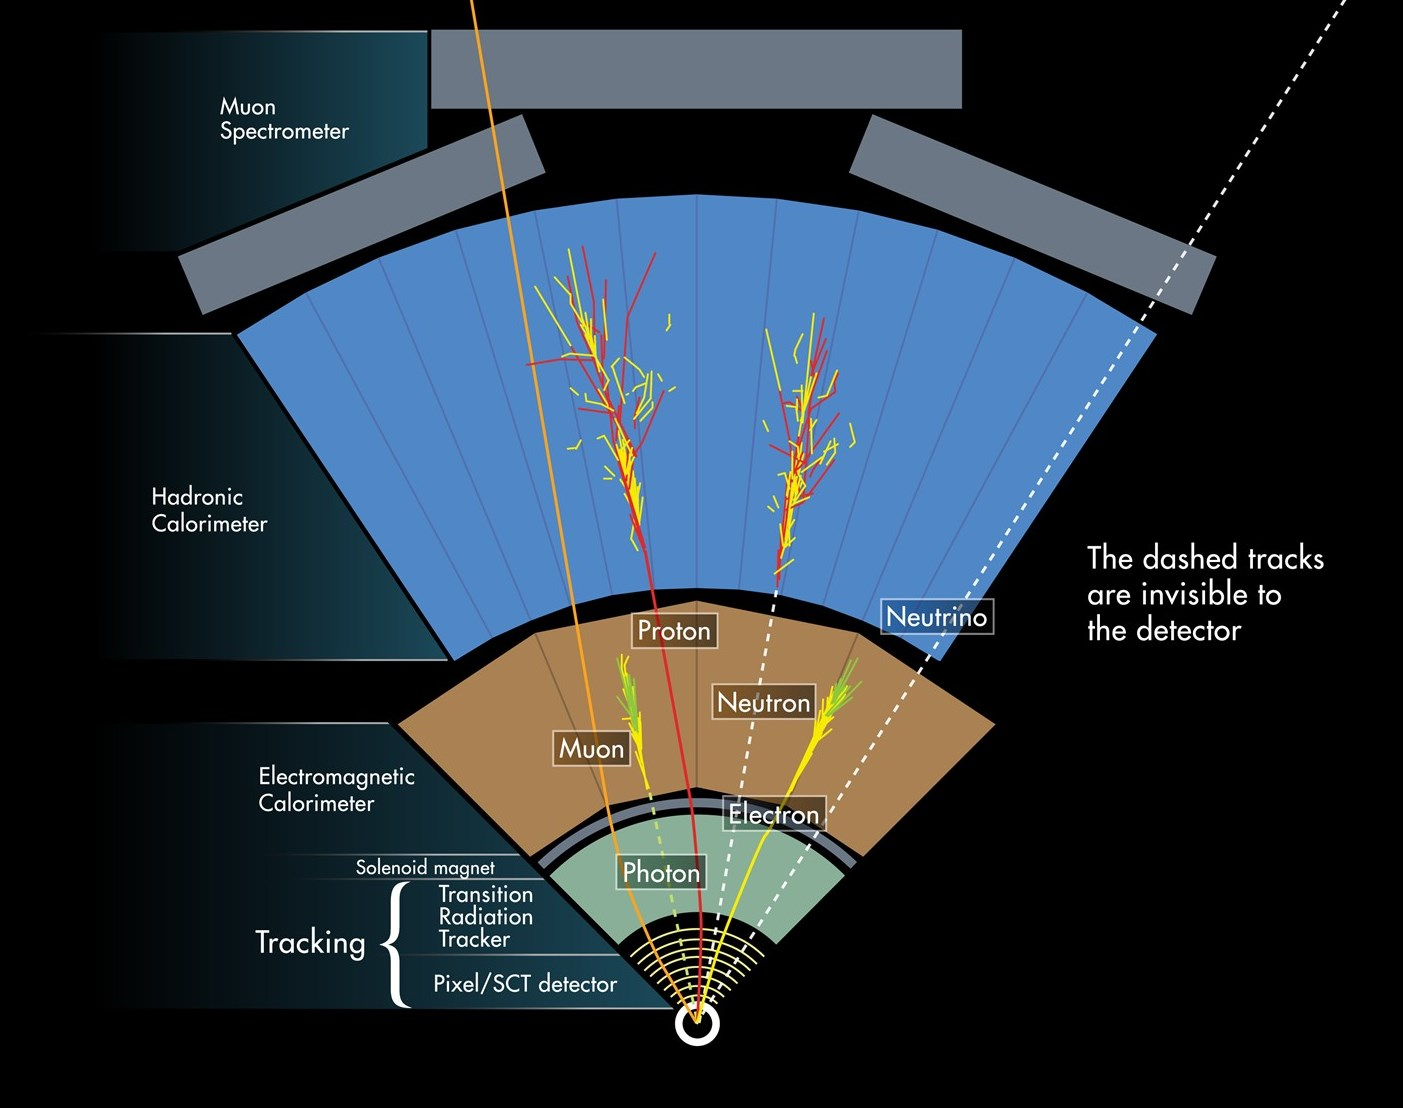
\includegraphics[width=\textwidth]{./figures/detector.jpg}
    }
\end{frame}
}

% -----------------------------------------------------------------------------

\begin{frame}{Data analysis tasks in detectors}
\begin{enumerate}

\item Track finding\\
    {\scriptsize Reconstruction of particle trajectories from hits in detectors}

    \vspace{0.5cm}

\item Budgeted classification\\
    {\scriptsize Real-time classification of events in triggers}

    \vspace{0.5cm}

\item Classification of signal / background events\\
    {\scriptsize Offline statistical analysis for discovery of new particles}

    \vspace{0.5cm}

\item ...

\end{enumerate}
\end{frame}

% -----------------------------------------------------------------------------

\begin{frame}{The Higgs Boson challenge (in HEP terms)}

\begin{itemize}
\item Data comes as a finite set $${\cal D} = \{(\X{\mathbf{x}_i}, \y{y_i}, \w{w_i}) | i = 0, \dots, N-1 \},$$
where \X{$\mathbf{x}_i \in \mathbb{R}^d$}, \y{$y_i \in \{\text{signal}, \text{background}\}$} and \w{$w_i \in \mathbb{R}^+$}.

\vspace{0.5cm}

\item The goal is to find a region ${\cal G} = \{ \X{\mathbf{x}} | \model{g}(\X{\mathbf{x}}) = \y{\text{signal}}\} \subset \mathbb{R}^d$, defined from a binary function \model{$g$}, for which
the background-only hypothesis can be rejected at a strong significance level ($p=2.87\times 10^{-7}$, i.e., \textit{5 sigma}).

\vspace{0.5cm}

\item Empirically, this is approximately equivalent to finding \model{$g$} from ${\cal D}$ so as to maximize $\text{AMS} \approx \frac{s}{\sqrt{b}}$, where
\begin{itemize}
    \item $s = \sum_{\{i | \y{y_i = \text{signal}}, \model{g}(\X{\mathbf{x_i}}) = \y{\text{signal}}\}} \w{w_i}$
    \item $b = \sum_{\{i | \y{y_i = \text{background}}, \model{g}(\X{\mathbf{x_i}}) = \y{\text{signal}}\}} \w{w_i}$
\end{itemize}

\end{itemize}
\end{frame}

% -----------------------------------------------------------------------------

\begin{frame}{The Higgs Boson challenge (in machine learning terms)}

Find a binary classifier

$$\model{g} : \X{\mathbb{R}^d} \mapsto \y{\{\text{signal}, \text{background}\}}$$

\vspace{0.25cm}

maximizing the objective function

$$AMS \approx \frac{s}{\sqrt{b}},$$

where
    \begin{itemize}
        \item $s$ is the \w{weighted} number of true positives
        \item $b$ is the \w{weighted} number of false positives.
    \end{itemize}
\end{frame}

% -----------------------------------------------------------------------------

\begin{frame}{Winning methods}

\begin{figure}
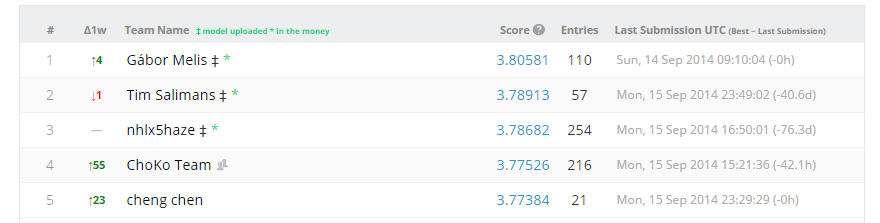
\includegraphics[width=\textwidth]{./figures/lb.png}
\end{figure}

\begin{itemize}
\item Ensembles of neural networks (1st and 3rd);
\item Ensembles of regularized greedy forests (2nd);
\item Boosting with regularization (XGBoost package).

\vspace{0.25cm}

\item Most contestants dit not optimize AMS directly;
\item But chosed the prediction cut-off maximizing AMS in CV.
\end{itemize}
\end{frame}

% -----------------------------------------------------------------------------

\begin{frame}{Lessons learned (for machine learning)}

\begin{itemize}
\item AMS is {\color{red} highly unstable}, hence the need for
    \begin{itemize}
        \item Careful, rigorous and stable cross-validation to avoid overfitting.
        \item Ensembles to reduce variance ;
        \item Regularized base models.
    \end{itemize}


\begin{figure}
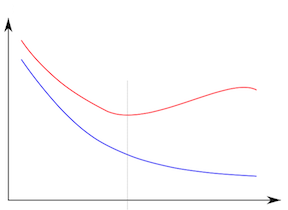
\includegraphics[scale=0.3]{./figures/overfitting.png}
\end{figure}

\item Support of samples weights \w{$w_i$} in classification models
      was key for this challenge.

\vspace{0.5cm}

\item Feature engineering hardly helped.

\end{itemize}

\end{frame}

\begin{frame}{Lessons learned (for physicists)}

\begin{itemize}
\item Domain knowledge hardly helped.

\vspace{0.25cm}

\item Standard machine learning techniques, run on a single laptop, easily beat HEP benchmarks.

\vspace{0.25cm}

\item Physicists started to realize that {\color{blue} collaborations with machine learning experts
    is likely to be beneficial}.

    \begin{itemize}
    {\scriptsize
    \item \textit{I worked on the ATLAS experiment for over a decade [...] It is rather depressing to see how badly I scored. -- Andrew John Lowe} \\
    \item \textit{The final results seem to reinforce the idea that the machine learning experience is vastly more important in a similar contest than the knowledge of particle physics. I think that many people underestimate the computers. -- Lubos Motl}
    \item \textit{It is probably the reason why ML experts and physicists should work together for finding the Higgs. -- phunter}
    }
    \end{itemize}

\end{itemize}



% enthousiasm towards unknown ML techniaues
% http://www.kaggle.com/c/higgs-boson/forums/t/10350/how-physicists-fared

% tMVA + ROOT, often considered as a black box
% simple statistical methods
% lack of adoption because understandable or because it works
% overall, the whole statistical and data ecosystem has been developed in vase clos
\end{frame}

% -----------------------------------------------------------------------------

\begin{frame}{Scientific software in HEP}

\begin{itemize}
    \item ROOT and TMVA are standard data analysis tools in HEP.

    \vspace{0.25cm}

    \item Surprisingly, this {\color{red} HEP software ecosystem proved to be rather limited
          and easily outperformed}, in the context of the Kaggle challenge.

    \vspace{0.25cm}

    \item Yet, the adoption of external solutions (e.g., the scientific Python ecosystem) appears to be slow and difficult because of
        \begin{itemize}
            {\scriptsize
            \item The effort of relearning new tools ;
            \item Lack of understanding of non-HEP methods ;
            \item Genuine ignorance.
            }
        \end{itemize}

    \begin{figure}
    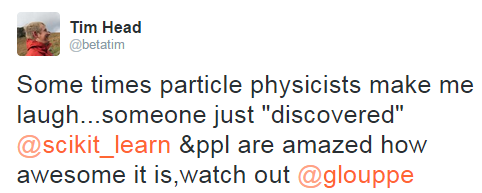
\includegraphics[width=0.5\textwidth]{./figures/tim.png}
    \end{figure}

\end{itemize}

\end{frame}

% -----------------------------------------------------------------------------

\begin{frame}{Scikit-Learn in Particle Physics?}

\begin{itemize}
\item The major blocker for the larger adoption of Scikit-Learn in HEP remains the {\color{red} full support of sample weights} throughout
      all essential modules.

      \begin{itemize}
        {\scriptsize
        \item Since 0.16, weights are supported in all ensembles and in most metrics.
        \item Next step is to add support in grid search. }
      \end{itemize}

      \vspace{0.5cm}

\item In parallel, domain-specific packages are getting traction

      \begin{itemize}
        {\scriptsize
        \item \texttt{ROOTpy}, for bridging the gap between ROOT data format and NumPy;
        \item \texttt{lhcb\_trigger\_ml}, implementing ML algorithms for HEP, on top of scikit-learn.}
      \end{itemize}

\end{itemize}

\end{frame}

% -----------------------------------------------------------------------------

\begin{frame}{Conclusions}

\begin{itemize}
\item Despite being known for being conservative, (some) physicists start
adopting the scientific Python ecosystem for exploratory data analysis.

\vspace{0.5cm}

\item Scikit-Learn has the potential to become an important tool in the field.

\vspace{0.5cm}

\item Overall, on both data analysis and software aspects, this calls
  for a {\color{blue} larger collaboration between data sciences and HEP}.
\end{itemize}

\vspace{0.25cm}

\begin{center}
\it The process of attempting as a physicist to compete against ML experts
has given us a new respect for a field that (through ignorance) none of us held in as high esteem as we do now.
\end{center}

\end{frame}

% -----------------------------------------------------------------------------

\appendix

\begin{frame}

\begin{figure}
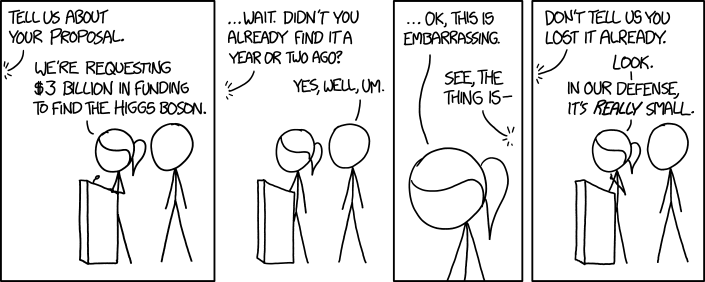
\includegraphics[width=0.9\textwidth]{./figures/xkcd.png}
\end{figure}

\vspace{0.5cm}

\begin{center}
{\Huge  Questions?}
\end{center}
\end{frame}

\end{document}
